\renewcommand{\theequation}{\theenumi}

\begin{theorem}\label{theorem:th1_quadilateral_ex}
Sum of opposite angles in a cyclic quadilateral equals $180\degree$.
\end{theorem}

\begin{enumerate}[label=\thesubsection.\arabic*.,ref=\thesubsection.\theenumi]
\numberwithin{equation}{enumi}

\item \solution  From theorem \ref{theorem:th1_quadilateral_ex}
\begin{align}
\angle A + \angle C &=  180\degree\\
\angle B + \angle D &=  180\degree
\end{align}

\item From the given information:
\begin{align}
4y+20-4x &= 180\degree \label{eq:sol1_quadilateral_ex} \\
3y-5-7x+5 &= 180\degree \label{eq:sol2_quadilateral_ex}
\end{align}

\item Solving equations \ref{eq:sol1_quadilateral_ex} and \ref{eq:sol2_quadilateral_ex}:
\begin{align}
x &= -15 \\
y &= 25 \\
\implies \angle A &= 120\degree \\
\implies \angle B &= 70\degree \\
\implies \angle C &= 60\degree \\
\implies \angle D &= 110\degree 
\end{align}


\item \begin{figure}[!ht]
\centering
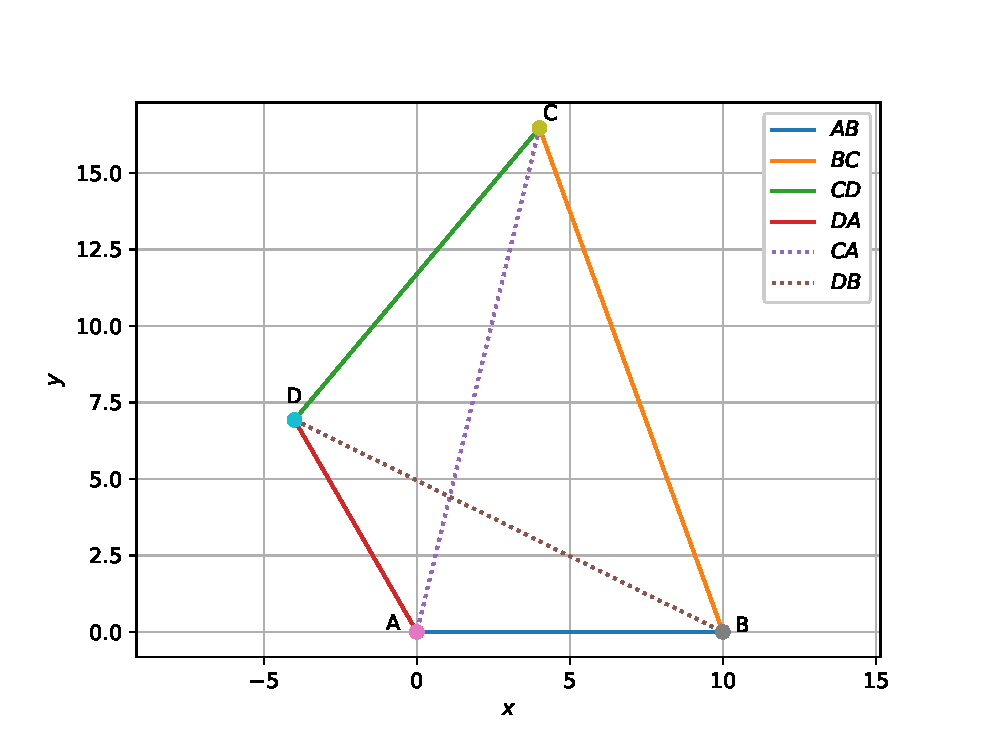
\includegraphics[width=\columnwidth]{./figs/quadilateral_ex/cyclic_quad.eps}
\caption{Quadilateral generated using python}
\label{fig:cyclic_quad2_quadilateral_ex}
\end{figure} 

The following Python code generates Fig. \ref{fig:cyclic_quad2_quadilateral_ex}

\begin{lstlisting}
codes/quadilateral_ex/cyclic_quad.py
\end{lstlisting}
\end{enumerate}



